\cotefile{148}
\scanpage{44}
\mspage{1}

\uline{Groupoïdes de Teichmüller}.

\textcircled{1} Cas topologique.

La variante la plus simple est
\[
{\unsure{\mathscr T|\mathbb T}}_{\mathrm{top}}^{+}\quad\text{ou}\quad\mathscr T_{\mathrm{top}}
\]
(\uline{groupoïde de Teichmüller \uline{orienté} topologique})

% slanted
\margin{Finalement, tant qu'on ne travaille pas au point de vue arithmétique, il semble que c'est le gros $\mathscr T^{\pm}$ qui sera le plus utilisé, \deleted{\unsure{tout|tant}} c'est lui qui mérite donc ici la notation la plus simple $\mathscr T$, et le \unsure{gr. or|groupe|gr.} orienté de s'appeler $\mathscr T^{+}$.}

\uline{Objets}: surfaces \uline{à bord} compactes orientées

\uline{flèches}: classes d'isotopie d'Iso conservant l'orientation)

Variante immédiate
\[
\mathscr T_{\mathrm{top}}^{\pm}
\]
(\uline{groupoïde de Teichmüller} \uuline{biorienté} \uline{topologique}): mêmes objets, flèches $=$ \deleted{les} classes d'isotopie d'homéomorphismes (ne conservant pas néc. l'orientation).

Soit $[\pm1]$ le groupoïde ayant un seul objet $e$ (par exemple $e=\varnothing$) et comme groupe d'autom. $\pm1$. On a un morphisme de signature
\[
\mathscr T_{\mathrm{top}}^{\pm}\xrightarrow{\unsure{\chi}}\,[\pm1]
\]
dont la \uline{fibre} \deleted{est} (ou noyau) est $\mathscr T_{\mathrm{top}}^{+}=\mathscr T_{\mathrm{top}}$.

% slanted
\margin{\unsure{canulé|calculé}, si on \unsure{ne} se borne à des surfaces connexes !}

La variante la plus complexe est
\[
S_{*}\mathscr T{\unsure{\mathbb D|D}}_{\mathrm{top}}^{+}\quad\text{ou}\quad S_{*}\mathscr T\mathbb D_{\mathrm{top}},
\]
``\uline{groupoïde de Teichmüller} \inserted{\uline{orienté}} \uline{spécial dévissé topologique}''
% archive sheet number: 43

\scanpage{45}
\deleted{On a ainsi la notion de \uline{graphe pondéré enrichi} (pondéré par $\unsure{\gamma|g}$, la structure}
% archive sheet number: 44

\scanpage{46}
\mspage{2}

\uline{Objets}: Triples $(X,\widetilde\Sigma,\deleted{\unsure{G|S}}R)$, avec

\margin{$X,\deleted{\partial X}\!,\Sigma,S$}

$X$ surface à bord compacte orientée

$\widetilde\Sigma$ sous-$1$-variété compacte de $X$ \deleted{$\unsure{\partial X}$}, $\widetilde\Sigma\supset\partial X$

\deleted{$\unsure{G|S}$} $R\subset\Sigma$ \deleted{$\unsure{\partial X}$}, partie finie

% slanted
\margin{$\widetilde\Sigma=\partial X\amalg\Sigma$. On peut considérer que $R$ rigidifie, \unsure{mais} aussi que $R$ ``découpe'' $\widetilde\Sigma$\ldots}

\uline{flèches}: classes d'isotopie d'homéom. conservant l'orientation

\deleted{Variante} \deleted{\unsure{on}} Les \unsure{comp.}\,\unsure{des|s.} connexes de $\widetilde\Sigma\setminus\partial X$ \inserted{$=\Sigma$} (\inserted{celles de $\partial X$ sont \uline{les cercles de raccord}}) sont les \uline{cercles de découpage}, les éléments de \deleted{$\unsure{G|S}$}$R$ sont les \deleted{\unsure{points marqués}} \uline{sommets de} \deleted{\unsure{marquage}} \inserted{\uline{rigidification}} \deleted{(ou de rigidification)}, \deleted{les composantes de $\partial X$ sont les ``trous''}. Les composantes connexes de $X$ sont les \deleted{\unsure{morceaux}} \inserted{\uline{composants}} de l'objet envisagé.

Variante $S_{*}\unsure{\mathscr T|\mathbb T}{\unsure{\mathbb D|D}}_{\mathrm{top}}^{\pm}$, avec
\diagram{\begin{tikzcd}[ampersand replacement=\&,column sep=large]
 S_{*}\mathscr T\mathbb D_{\mathrm{top}}\arrow[r,hook,no head] \& S_{*}\mathscr T\mathbb D_{\mathrm{top}}^{\pm}\arrow[r] \& {[\pm1]}
\end{tikzcd}}
comme tantôt.

On a des sous-groupoïdes pleins

\diagram{\(\begin{array}{llll}
\deleted{\unsure{G}=\Sigma=\varnothing}\;\inserted{R=\varnothing,\Sigma=\varnothing}
 &\mathscr T_{\mathrm{top}} &\text{et } \mathscr T_{\mathrm{top}}^{\pm} &\\
\substack{\Sigma=\deleted{\unsure{\partial X}}\varnothing\\ R\text{ quelconque}}
 &S_{*}\mathscr T_{\mathrm{top}} &\text{et }S_{*}\mathscr T_{\mathrm{top}}^{\pm}
 &\substack{\text{(groupoïdes de Teichmüller }\text{\uline{spéciaux}}\\
 \text{\inserted{(ou \uline{rigidifiés})}}\\\text{(topologique orienté)}}\\
 \deleted{\unsure{S}}R=\varnothing
 &\mathscr T\mathbb D_{\mathrm{top}} &\text{et }\mathscr T\mathbb D_{\mathrm{top}}^{\pm}&
\end{array}\)}

(Cas pas intéressant je crois, sauf pour $\Sigma=\varnothing$ également)

% slanted
\margin{$MD={}$``\unsure{modulPair|modulaire}'' ou Mumford-Deligne}

\deleted{\unsure{Dé}} \uline{Détermination} du $\pi_0(S_{*}\mathscr T\mathbb D_{\mathrm{top}})\xrightarrow{\sim}\pi_0(S_{*}\mathscr T\mathbb D_{\mathrm{top}}^{\pm})$.

On introduit les \uline{graphes} \deleted{\unsure{MD}} bipondérés
% archive sheet number: 45

\scanpage{47}
\mspage{3)}

qui forment un groupoïde \deleted{\unsure{$MD$}}. $\mathrm{Grbip}$ \deleted{\unsure{ou}} $(\mathrm{Grabipond})$

Objets : graphes \inserted{finis} $(S,\vec A,\sigma,o)$ \inserted{$+$ structure suppl.} (pouvant avoir des sommets isolés, des boucles fermées, a fortiori plusieurs arêtes entre deux sommets, et aussi des ``\uline{arêtes libres}'' correspondant aux pts fixes de $\sigma$)

% slanted
\margin{pas assez \unsure{précis|précisé} comme donnée. --- La pondération d'une arête doit être remplacée par celle d'un pol. comb. $T_a$ avec $\unsure{\omega(T_a)\simeq a|\mathrm{or}(T_a)\simeq a|n(T_a)\simeq a}$.}

$S,\vec A$ ens. finis \inserted{(``sommets'', ``arcs'')}, $\sigma:\vec A\unsure{-|\to}\vec A$ involution, $o:\vec A\to S$ appl\textsuperscript{n} ``origine''. On se donne de plus

\margin{J'ai indiqué une pondération des sommets, mais pas des arêtes}

\figure{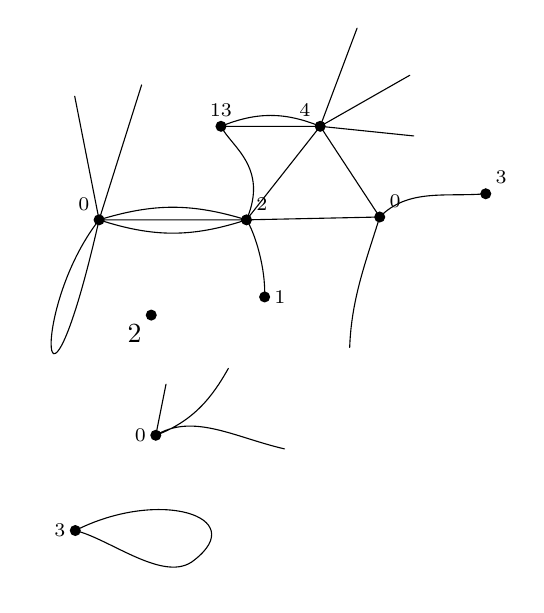
\begin{tikzpicture}[x=.72cm,y=.72cm,line cap=round]
\coordinate (a) at (0,2); \coordinate (b) at (2.6,2); \coordinate (c) at (2.15,3.65);
\coordinate (d) at (3.9,3.65); \coordinate (e) at (4.95,2.05);
\draw (a) to[bend left=17] (b) (a)--(b) (a) to[bend right=18] (b);
\draw (a) .. controls (-1.25,.4) and (-1.0,-2.4) .. (a);
\draw (a)--(-.43,4.18) (a)--(.75,4.38);
\draw (b) .. controls (3.0,2.93) and (2.32,3.3) .. (c);
\draw (c)--(d) (c) to[bend left=22] (d) (b)--(d)--(e)--(b);
\draw (d)--(4.55,5.38) (d)--(5.48,4.55) (d)--(5.55,3.48);
\draw (e).. controls (4.7,1.25) and (4.45,.6) ..(4.42,-.25);
\draw (e).. controls (5.45,2.56) and (6.12,2.4) ..(6.82,2.46);
\draw (b) .. controls (2.75,1.77) and (2.94,1.15) ..(2.92,.64);
\foreach \p/\lab/\where in {a/0/above left,b/2/above right,c/13/above,d/4/above left,e/0/above right}
 {\fill (\p) circle (2pt) node[\where] {\scriptsize $\lab$};}
\fill (6.82,2.46) circle (2pt) node[above right]{\scriptsize $3$};
\fill (2.92,.64) circle (2pt) node[right]{\scriptsize $1$};
\fill (.92,.32) circle (2pt) node[below left]{$2$};
\draw (1,-1.8)--(1.18,-.9) (1,-1.8) .. controls (1.67,-1.55) and (2,-1.12) ..(2.28,-.62)
 (1,-1.8).. controls (1.66,-1.4) and (2.4,-1.84) ..(3.27,-2.04);
\fill (1,-1.8) circle (2pt) node[left]{\scriptsize $0$};
\draw (-.42,-3.48) .. controls (1.06,-2.73) and (2.67,-3.23) ..(1.68,-4.0) .. controls (1.17,-4.43) and (.2,-3.63) ..(-.42,-3.48);
\fill (-.42,-3.48) circle (2pt) node[left]{\scriptsize $3$};
\end{tikzpicture}}

\[
 S\xrightarrow{\deleted{\unsure{g}}\gamma}\mathbb N\qquad\text{(application ``genre'' ou ``poids'')}
\]

\[
 \deleted{\unsure{\vec A^{\sigma}}=}\widetilde A \xrightarrow{r\,\deleted{\unsure{\rho_2|\rho z}}}\mathbb N
 \qquad\text{(application \deleted{\unsure{rigi}}\deleted{\unsure{de marquage et}} ``indice de rigidification'')}
\]
\deleted{``\unsure{ensemble des arêtes libres}''}
\[
 \widetilde A\overset{\text{déf}}{=}\vec A/\sigma
\]

\deleted{Ou encore, posant $\widetilde S=S\amalg A_l$, (identifié à l'ens. de \uline{tous} les ``sommets'', \inserted{apparents} \deleted{\unsure{marqués}} et \uline{``masqués''} (i.e. $\unsure{\in S|\notin S}$) \inserted{et fictifs (ces d. correspondant aux $\in A_l$)} du graphe), on donne}
\[
 \deleted{\widetilde S\xrightarrow{\pi}\mathbb N}\qquad\text{(\uline{pondération} du graphe)}
\]
\deleted{``\unsure{ens. des sommets apparents}''}

\margin{$\widetilde S=S\amalg\deleted{\unsure{S_l}}{}\underset{\shortparallel}{\unsure{S_l}}$ \deleted{\unsure{sommets fictifs}}\\ $A_l$}

La donnée du \uline{graphe} sous-jacent à un graphe \deleted{$MD$} \inserted{bip.} revient à celle du graphe ``ordinaire'' correspondant (sans arêtes \uline{libres}, i.e. où $\sigma$ opère sans pts fixes), i.e.
\[
 (S,(\vec A\setminus\vec A^\sigma),\sigma|(\vec A\setminus\vec A^\sigma),o|{\vec A\setminus\vec A^\sigma}),
\]
\uline{plus} un ensemble \inserted{fini} $A_l$ (\deleted{\unsure{sommets}} \inserted{arêtes} libres) \deleted{ou ``sommets-trous'')} et une application
\[
 A_l\longrightarrow S
\]

\margin{$\widetilde A=\vec A/\sigma=A\amalg A_l$}

\diagram{\begin{tikzcd}[ampersand replacement=\&,row sep=large,column sep=small]
\vec A \arrow[d]\arrow[d,shift right=1.5,no head,"\deleted{\unsure{\pi}}"'] \& {}={} \&
\underbrace{\vec A_{0}}_{\vec A\setminus\vec A^\sigma}\arrow[d,"\mathrm{deg}\,2"]
 \& {}\amalg{} \& \underbrace{\vec A_l}_{\vec A^\sigma}\arrow[d,"\mathrm{deg}\,1"]\\
\widetilde A \& {}={} \& A \& {}\amalg{} \& A_l
\end{tikzcd}}

\margin{Ordre d'un sommet\\ $\sigma(s)=\underbrace{\sigma_l(s)}_{\substack{\text{correspond}\\\text{aux ``trous''}\\\text{ou cercles}\\\text{de recollage}}}+\sigma_{\unsure{0|o}}(s)$}

\uline{Flèches} \qquad les iso. de telles structures
% archive sheet number: 46

\scanpage{48}
\mspage{4)}

On a un foncteur
\[
 \Gamma:\quad S_{*}\unsure{\mathscr T|\mathbb T}{\unsure{\mathbb D|D}}_{\mathrm{top}}^{\pm}
 \longrightarrow\deleted{\unsure{\Gamma MD}}(\mathrm{Grabipond})\tag*{$(*)$}
\]
qui associe à un objet \inserted{$(X,\widetilde\Sigma,R)$} de $S\mathscr T\deleted{\unsure{D}}\mathbb D_{\mathrm{top}}^{\pm}$ le graphe \inserted{$MD$} $(S,\vec A,\sigma,\deleted{\unsure{r|k}}o,\deleted{\unsure{g}}\gamma,\rho)$ suivant :

\[
 S=\pi_0(X\deleted{\unsure{,}}\setminus\widetilde\Sigma)\xleftarrow{\sim}\pi_0(\mathrm{Déc}(X,\widetilde\Sigma))
\]

$\vec A={}$ ens des couples $(C,\deleted{\unsure{g}}\omega)$, où $C$ \deleted{est un} \inserted{$\in\pi_0(\widetilde\Sigma)$}, et où $\omega\in\mathrm{Or}(C)$ \inserted{$\simeq\mathrm{rive}_{X}(C\deleted{\unsure{,}})$}, soumis à la condition que si $C\in\pi_0(\partial X)$, alors $\omega$ soit l'orientation induite i.e. la rive qui se trouve dans $X$

$\sigma={}$ échange des rives (quand on a le droit d'échanger, sinon, i.e. si \unsure{$^{a}$}$C\in\pi_0(\partial X)$, on pose $\sigma(a)=a$)

\deleted{$\unsure{R\to R}$} $o\deleted{\unsure{(a)}}:$ associe à $(C,\text{rive de }C)$ l'unique ``face'' $\in\pi_0(X\setminus\widetilde\Sigma)$ qui contient cette rive

\[
 \gamma:\underset{\substack{\shortparallel\\\pi_0(X\setminus\widetilde\Sigma)}}{S}\longrightarrow\mathbb N
 \qquad\text{application \uline{genre} du composant $\unsure{X'|X_i|X_s}$.}
\]

\[
 \deleted{\unsure{\rho}}r:\quad A=\pi_0(\widetilde\Sigma)\longrightarrow\mathbb N:\quad C\longmapsto\mathrm{Card}(R\cap C).
\]

Le foncteur $(*)$ \deleted{est \uline{ess. surjectif} et} \inserted{induit un \uline{iso} sur les} $\pi_0$ et \unsure{une|un} surjectif sur les $\pi_1$ (c'est un \uline{$0$-isomorphisme} \deleted{\unsure{)}}, en langage homotopique).

\deleted{\unsure{Prop.}} \deleted{\unsure{Les obj.}}

\uline{Remarques} \quad Dans $S_{*}\mathscr T\mathbb D_{\mathrm{top}}^{\pm}$ il y a une opération évidente de \uline{sommes} \inserted{\uline{directes}}, dans \deleted{$\Gamma MD$} $\mathrm{Grabipond}$ aussi, et $(*)$ y commute.
% archive sheet number: 47

\scanpage{49}
\mspage{5)}

Cette opération de \unsure{somme|sommes} est la plus triviale parmi les opérations qu'il nous faudra expliciter et transcrire (combinatoirement) dans la suite. Notons de suite, pour $(X,\widetilde\Sigma,R)$\deleted{\unsure{,}} donné
\[
 X\,\deleted{\unsure{\ne}}\ \text{connexe}\quad\Longleftrightarrow\quad\Gamma MD(X,\widetilde\Sigma,R)\ \text{connexe}
\]
plus précisément
\[
 \pi_0(X)\simeq\pi_0(\Gamma MD(X,\widetilde\Sigma,R))
\]

% slanted
\margin{donner la formule pour le genre d'un $\alpha\in\pi_0(X)\simeq\pi_0(\Gamma)$ en termes de la pondération $g_s$ --- plus généralement, le \uline{genre total} est donné par $g=\sum_{s\in S}g_s+c(\Gamma)$}

% slanted
\margin{``indice de connexion'' du graphe $=\deleted{\unsure{\chi(\Gamma)}}\unsure{\mathrm{rg}}\ H_1(\Gamma)$}

\uline{Cas particuliers}.

a) Cas de $S_{*}{\unsure{\mathscr T|\mathbb T}}_{\mathrm{top}}^{\pm}$ \deleted{$\unsure{S\mathscr T_{\mathrm{top}}}$} --- \unsure{i.e.|ici|idem} $\Sigma=\varnothing,\ \widetilde\Sigma=\partial X$.

Cela \unsure{correspond} au cas des graphes $MD$ \deleted{qui} où \inserted{toutes les arêtes sont libres, i.e.,} tous les sommets sont isolés (sauf arêtes libres)

\deleted{Elle} \inserted{Ce graphe} est \deleted{une} déterminé par
\diagram{\begin{tikzcd}[ampersand replacement=\&,column sep=large]
 A\;(=\vec A=\vec A^\sigma)\arrow[d]\arrow[r,"r"] \& \mathbb N\\
 S\arrow[r,"\gamma"] \& \mathbb N
\end{tikzcd}}

Le cas de $\mathscr T_{\mathrm{top}}^{\pm}$ correspond à celui où $\rho=0$, donc la situation est donnée par
\diagram{\begin{tikzcd}[ampersand replacement=\&]
 A=A_0\arrow[d]\&\\
 S\arrow[r,"\gamma"]\&\mathbb N .
\end{tikzcd}}

\figure{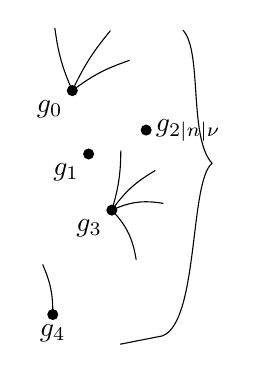
\begin{tikzpicture}[x=.67cm,y=.66cm,line cap=round]
\draw (.6,3.6) to[bend left=8](.27,4.8) (.6,3.6) to[bend left=7](1.32,4.75) (.6,3.6) to[bend left=9](1.68,4.18);
\fill (.6,3.6) circle (2pt) node[below left]{$g_0$};
\fill (.91,2.38) circle (2pt) node[below left]{$g_1$};
\fill (2.0,2.84) circle (2pt) node[right]{$g_{\unsure{2|n|\nu}}$};
\draw (1.35,1.3) to[bend right=8](1.52,2.44) (1.35,1.3) to[bend left=12](2.17,2.06)
 (1.35,1.3) to[bend left=17](2.32,1.43) (1.35,1.3) to[bend left=17](1.81,.35);
\fill (1.35,1.3) circle (2pt) node[below left]{$g_3$};
\draw (.23,-.71) to[bend right=12](.04,.25); \fill (.23,-.71) circle (2pt) node[below]{$g_4$};
\draw (2.7,4.76).. controls (3.07,4.35) and (2.8,2.7)..(3.25,2.2)
 .. controls (2.82,1.86) and (3,-.85)..(2.31,-1.12)--(1.51,-1.28);
\end{tikzpicture}}

\deleted{type $(g,\nu)$ d'une \unsure{surface}} Le cas d'une structure connexe ($\mathrm{card}.S=1$ \inserted{i.e. $S=\{s\}$}) est \deleted{\unsure{donné par la donnée}} \inserted{caractérisé par la donnée} des deux entiers $(g,\nu)$ \quad ($g=$ genre, $\nu={}$ nb de trous)
\[
 g=\gamma(s),\quad \nu=\mathrm{card}\,A
\]
% archive sheet number: 48

\scanpage{50}
\mspage{6}

\uline{Remarques} \quad En fait, on a un foncteur plus précis, vers une catégorie de graphes munis d'une structure où la partie $\rho$ de la pondération est \deleted{\unsure{complétée}} \deleted{\unsure{remplacée}} \inserted{remplacée} par une structure plus précise, à savoir \deleted{une application} \inserted{une \deleted{\unsure{appli}} famille}
\[
 \deleted{\unsure{A}\;(\widetilde R,\alpha,p:R\to\underset{\substack{\shortparallel\\\vec A/\sigma}}{\vec A})}\quad (R_a)_{a\in A}
\]
d'ensembles, et pour tt $a\in A$, si $\omega(a)$ désigne l'ens. des \deleted{où $\alpha$ est une involution sans points fixes de} \deleted{des} ``orientations'' de $a$ (card $\omega(a)\in\{1,2\}$), une application

% slanted
\margin{$\omega(a)\overset{\mathrm{def}}{=}\{\vec a\in\vec A\,/\,\vec a\ \text{au dessus de }a\}$}

\deleted{$R$, et $p$ une application $R\to A$ comp. avec $\alpha$}
\[
 \omega\longmapsto u_\omega:\quad \omega(a)\longrightarrow\mathrm{Circ}(R_a)
 \quad\text{ens des permutations circulaires sur $R_a$}
\]
\deleted{et induisant \unsure{une iso.} une application \uline{injective}}
\[
 \deleted{R/\alpha\lhook\joinrel\longrightarrow\vec A}
\]
avec la condition que si $\omega,\omega'\in\omega(a)$, $\omega\ne\omega'$, alors $\deleted{u_\omega u_{\omega'}=\mathrm{id}_{R_a}}\quad u_{\omega'}=u_\omega^{-1}$

On peut aussi considérer que la donnée supplémentaire revient à la donnée de
\[
 \begin{aligned}
 r:&\quad A\longrightarrow\mathbb N\\
 \shortparallel&\\[-4pt]
 a&\longmapsto\mathrm{Card}\,p^{-1}(a)
 \end{aligned}
\]
(la ``pondération-arêtes''), et la donnée d'une famille de torseurs
\[
 (R_a)_{a\in A},\ \deleted{\unsure{r(a)>0}}
\]
$R_a$ un torseur sous $\mathbb Z/r(a)\mathbb Z\mathbin{\underset{\{\pm1\}}{\wedge}}^{\omega(a)}$. On associe à $(X,\widetilde\Sigma,R)$ une telle structure supplémentaire où
\[
 R_a=R\cap\widetilde\Sigma_a
 \qquad\text{($\widetilde\Sigma_a$ la comp. connexe de $\widetilde\Sigma$ \deleted{\unsure{au point}} qui correspond à $a\in A\simeq\pi_0(\widetilde\Sigma)$)}
\]
\deleted{$R=R$ (sic), $R\longrightarrow\underset{\substack{\shortparallel\\\pi_0(\Sigma)}}{S}$ déduit de $R\subset\Sigma$}

$\omega\mapsto u_\omega$ défini de façon \unsure{adéquate|évidente}.

et \deleted{$p$ déduit de l'ordre circulaire sur les $R_a$}

\uline{NB} Même si $r(\omega)=1$ ou $\unsure{r(\omega)|\text{même}}=2$, le fait de disposer
% archive sheet number: 49

\scanpage{51}
\mspage{\deleted{\unsure{6}}7}

d'une structure déjà orientée si $a$ est une arête libre (correspondant à un $C\in\pi_0(\partial X)$), ou qu'on dispose de l'\deleted{\unsure{une|ens}} des deux orientations $\omega(a)$ \deleted{\unsure{=}} dans le cas où $a$ est une arête ordinaire, implique que l'on tient en mains, pour chaque $a\in A$, un polygone combinatoire $P_a$, dont l'ens des sommets est $R_a$, et l'ens des arêtes peut se décrire \deleted{\unsure{comme}} de façon canonique en termes de $R_a,\omega_a$ et $\omega_a\to\mathrm{Circ}(R_a)$. Il peut être plus commode de la donner d'emblée dans la structure, \deleted{qui serait alors un contour} \inserted{où la famille des $\unsure{R_a|P_a}$ serait \unsure{renforcé|remplacé} par un} \uline{contour combinatoire}, i.e. un ensemble de repères $\underline{\vec R}$ (dits ``repères de rigidification''), avec une opération de
\[
 {\unsure{\mathbb D|D}}_{\infty}=\{\sigma_0,\sigma_1\mid\sigma_0^2=\sigma_1^2=1\}
\]
dessus, et une application
\[
 \underline{\vec R}\longrightarrow\vec A
\]
compatible avec l'hom
\[
 \mathbb D_{\infty}\xrightarrow{\unsure{\varepsilon|2}}\{\pm1\}
\]
sur les groupes d'opérateurs, mais de plus un sous ens
\[
 \underline{\vec R}_{l}^{+}\subset\underline{\vec R}\mid\vec A_l
\]

\margin{($\vec A_l={}$ arêtes libres, correspondant aux cercles de \unsure{recollement|recollements}, i.e. les $\in\pi_0(\deleted{\unsure{\partial}}\partial X)$)}

définissant une orientation du contour correspondant.
% archive sheet number: 50

\scanpage{52}
\mspage{8}

On a ainsi la notion de \uline{graphe pondéré} \deleted{\unsure{enrichi}} \uline{à repères} $\unsure{\Gamma|r}$

\margin{Groupoïde $(\uline{\mathrm{Gr.pondrep}})$\\ foncteur\\ $S_{*}\unsure{\mathscr T|\mathbb T}{\unsure{\mathbb D|D}}_{\mathrm{top}}^{\pm}\longrightarrow(\mathrm{Gr\,pond\,rep})$}

\diagram{\begin{tikzcd}[ampersand replacement=\&,column sep=small]
{\vec R_l^{+}\ \deleted{\mathbb D_\infty}\subset\underset{\sigma_0,\sigma_1}{\vec R}}\arrow[r] \&
\vec A\arrow[loop right,"\sigma"]\arrow[d,"o"']\&\\
\&S\arrow[r,"\gamma"]\&\mathbb N
\end{tikzcd}}

qui sera importante sans doute dans l'explicitation de l'opération de ``vrillement''. Il est clair en tous cas que toute description-traduction algébrico-combinatoire de $\unsure{S\mathscr T|\mathscr T}\mathbb D_{\mathrm{top}}^{\pm}$ devra permettre, pour chaque objet du \deleted{la catégorie} \inserted{groupoïde-}paradigme, de réconstituer (à isom. unique près) le \uline{graphe pondéré à repères} correspondant.

\inserted{--- plus précisément, il faut réconstituer le foncteur canonique $S_{*}\mathscr T\mathbb D_{\mathrm{top}}^{\pm}\longrightarrow(\mathrm{Grpondrep.})$ (et non seul\textsuperscript{mt} le foncteur à valeurs dans $(\mathrm{Grbipond})$)}

\uline{Opérations essentielles}

A) Opérations ``d'oubli'' ou de ``\uline{gommage}''.

\textcircled{1} \uline{Gommage de repères} \quad \unsure{A'|À} un objet $(X,\Sigma,R)$, muni en plus d'une partie $R'\subset R$, il associe $(X,\Sigma,R\setminus R')$ (gommage de $R'$).
% archive sheet number: 51

\scanpage{53}
\mspage{9}

\uline{NB} Ayant (via un groupoïde équivalent \deleted{\unsure{à}} \unsure{description|de conception} purement combinatoire) ``reconstruit'' ou \deleted{\unsure{remplacé}} réalisé le groupoïde $S\unsure{\mathscr T|\mathbb T}{\unsure{\mathbb D|D}}_{\mathrm{top}}^{\pm}$, et le foncteur
\[
 S\mathscr T\mathbb D_{\mathrm{top}}^{\pm}\longrightarrow(\mathrm{Gr.\ pond.\ rep})
\]

% slanted
\margin{\uline{NB} Cette opération a l'air d'un \uline{affaiblissement} de structure --- mais \unsure{elle|ce} n'est affaiblissement, sur une composante $C$ donnée de $\Sigma^+$, que lorsqu'on ``gomme'' \uline{tous} les repères de $C$ --- sinon c'est au contraire plutôt dans la nature d'un renforcement de structure, --- ou plutôt, du moment qu'on se donne déjà $R'_C=R'\cap C$, dans les catégories isotopiques \unsure{peu importe}, l'opération de gommage et celle \deleted{\unsure{au sens où}} de \unsure{surmarquage|sous-marquage} (cf plus bas) \unsure{correspondantes|corresp.} sont inverses l'une de l'autre, et sont des équivalences de groupoïdes. Il faudrait séparer les deux cas, pour distinguer les \uline{opérations de gommage essentielles} (qui changent \unsure{les groupes|le groupe} des automorphismes) et les autres.}

\deleted{\unsure{cela}} on aura \deleted{\unsure{par}} donc aussi \deleted{une traduction} \inserted{l'équivalent de} \deleted{de} la donnée d'un $(X,\Sigma,R)$, muni \uline{en plus} d'une partie $R'\subset R$ --- \deleted{\unsure{d'où}} i.e. \unsure{on va|on a|on aura} la construction d'un groupoïde \unsure{classifiant|fibrant}
\diagram{\begin{tikzcd}[ampersand replacement=\&]
 S_{*}\mathscr T\mathbb D_{\mathrm{top}}^{\pm}\ \text{(à sous ens. marqué $R'$ de sommets-repères)}\arrow[d]\\
 S_{*}\mathscr T\mathbb D_{\mathrm{top}}^{\pm}
\end{tikzcd}}

et \deleted{\unsure{d'où}} il nous faudra donc \inserted{décrire} un foncteur ``gommage de $R'$''
\diagram{\begin{tikzcd}[ampersand replacement=\&,column sep=large]
 S_{*}\mathscr T\mathbb D_{\mathrm{top}}^{\pm}\bigl(\underset{\text{marqué}}{\overset{\text{sous}}{\deleted{\unsure{R}}R'}}\bigr)
 \arrow[r,"\text{gommage de }R'", "\scriptstyle\rightarrow"{description,pos=.53,inner sep=0pt}]\&S_{*}\mathscr T\mathbb D_{\mathrm{top}}^{\pm}
\end{tikzcd}}

\deleted{Cela s'exprime, sur le} donnant lieu à un diagramme comm. de foncteurs

\diagram{\begin{tikzcd}[ampersand replacement=\&,column sep=small,row sep=small]
S_{*}\mathscr T\mathbb D_{\mathrm{top}}^{\pm}(\ldots R'\ldots)
 \arrow[rr,"\text{gommage de }R'"]\arrow[d,"\text{oubli du }\unsure{\text{marquage}|\text{sous-groupe}|\text{distinguage}}\ R'"] \& \& S_{*}\mathscr T\mathbb D_{\mathrm{top}}^{\pm}\arrow[ddl]\\
S_{*}\mathscr T\mathbb D\deleted{\unsure{R}}_{\mathrm{top}}^{\pm}\arrow[dr] \& \&\\
\&(\mathrm{Gra}\deleted{\unsure{\mathrm{bi}}}\mathrm{pond})\arrow[r] \& \substack{\text{graphes avec}\\\text{pondération}\\\text{par $\gamma$, mais}\\\text{non par $r$,}}
\end{tikzcd}}

alors qu'au niveau
% archive sheet number: 52

\scanpage{54}
\mspage{10}

des graphes pondérés à repères, l'opération \deleted{s'explicite} se reflète par une opération correspondante au niveau de $\vec R$, par le ``gommage'' d'une partie $\vec R'$ stable par ${\unsure{\mathbb D|D}}_\infty$ i.e. par $\sigma_0,\sigma_1$

2) Gommage de cercles de découpage

On se donne maintenant une \deleted{ens. de composantes connexes de} $1$-sous-variété \inserted{(ouv. et) fermée} $\Sigma'$ de $\Sigma\setminus\partial X$, correspondant à un ensemble \deleted{\unsure{des}} de \unsure{comp.} conn. de $\unsure{\Sigma'|\Sigma}$ i.e. à une partie \inserted{$A'_0$} de $\pi_0(\Sigma')=A_0$ (arêtes ordinaires du graphe) --- et on remplace $\Sigma$ par $\Sigma\setminus\Sigma'$. Au niveau du graphe pondéré, cela se traduit par une opération \uline{de contraction} \uline{en un point} des arêtes correspondantes, d'où formation d'un nouveau graphe, et d'un \uline{morphisme} \uline{de générisation} (à l'opposé de ``spécialisation'') de l'ancien vers le nouveau. Il convient ici d'expliciter comment la pondération suit\ldots\ Au niveau des \inserted{sommets-}repères, il est entendu que les sommets repères se trouvant sur $\Sigma'$ sont gommés en $=$ temps --- donc, sur le graphe pondéré à repères, on fait sauter l'ens des repères qui sont au dessus des arêtes $\in A_{\unsure{0|o}}'$.
% archive sheet number: 53

\scanpage{55}
\mspage{11}

3) \deleted{Gommage} \inserted{Bouchage de trous, ou ``gommage''} de cercles de recollement.

Cette opération est relative à la donnée d'une $1$-sous-variété fermée de $\partial X$, i.e. d'une partie $A'_l$ de $\pi_0(\partial X)\simeq A_l$ (ens des arêtes libres du graphe). Elle consiste à boucher les trous correspondants, au moyen \unsure{des|de} cônes sur les composantes connexes du bord de $\Sigma'_l$. Au niveau du graphe, cela consiste à gommer les arêtes libres correspondantes, avec bien entendu aussi les repères de marquage qui se trouvent au dessus --- \deleted{mais} les pondérations des \unsure{sommet|sommets} restent inchangées.

\deleted{\unsure{4)}} \uline{Gommage simultané mixte}, \deleted{\unsure{au}} correspondant à une partie \deleted{$A'\amalg R'$} \inserted{$R'\amalg\Sigma'$} \deleted{quelconque} de $R\amalg\Sigma$ \deleted{\unsure{du}} \deleted{\unsure{de} $A\amalg R$,} \inserted{qui soit à la fois ouverte et fermée} \deleted{i.e.} \inserted{et telle que $R'\supset R\cap\Sigma'$,} \deleted{une \unsure{ens.} de composantes connexes de $R\amalg\Sigma$,} ou ce qui revient au $=$, une partie \inserted{$R'\amalg A'$} de $R\amalg A$, telle que $R'\supset R|A'$. Au niveau du graphe pondéré à repères, cette opération consiste à enlever \deleted{\unsure{les}} \inserted{de $\vec R$} la partie corr. $\vec R'$, à contracter en un point les arêtes de $\unsure{A'|\Pi'}$\deleted{\unsure{pas}} (aussi bien libres que liées), en faisant suivre \unsure{les pondérations|la pondération}.
% archive sheet number: 54

\scanpage{56}
\mspage{12}

\deleted{\fbox{\unsure{4)}}} \inserted{(B)} \uline{Opération} \uline{de}\deleted{\uline{\unsure{affaiblissement|faiblissement} et de}} \inserted{sur}\uline{marquage}

\deleted{On peut la définir \deleted{par} \inserted{en termes de} la donnée, d'un pour chaque \deleted{arête du contour $R$} \inserted{composante connexe de} $\deleted{\unsure{R\times S}}\ \widetilde\Sigma\setminus R$ Soit $\deleted{\unsure{\widetilde\Sigma_*}}A_{\unsure{0|*}}^+$ eff. l'ens}

\deleted{\unsure{des a}} Soit $A^+$ l'ens des arêtes \inserted{(libres ou liées)} ``effectivement marquées'', \inserted{\unsure{de|du} $\Gamma$, \unsure{i.e.|p.ex.} telles que $r(a)>0$} \deleted{et $B$ ens des}, correspondant à des $C\in\pi_0(\Sigma)$ telles que $C\cap R\ne\varnothing$, soit $B^+$ l'ens des comp. connexes de $\Sigma^+\setminus R\cap\Sigma^+$ (lesquelles sont des int. ouverts), un surmarquage est défini par la donnée d'une application
\[
 B^+\xrightarrow{r'}\mathbb N,
\]

% slanted
\margin{\deleted{arêtes} cercles \deleted{\unsure{marqués}} \inserted{effectivement} marqués, \uline{arêtes} \inserted{\unsure{corr.}} sur $\Sigma$ (\uline{NB} elles se trouvent sur des cercles eff. marqués, et sont des intervalles ouverts)}

et peut se décrire \deleted{par} \inserted{comme} l'opération qui sur chaque \uline{arête} \inserted{(ouverte)} \deleted{qui} de $\Sigma$, correspondant à \unsure{un|une} $b\in B^+$, $r'(b)$ nouveaux sommets de \deleted{marquage} \inserted{rigidification}. Cette fois-ci, \deleted{\unsure{l'opéra}} il y a des choix arbitraires --- néanmoins l'opération donne un objet de $S\unsure{\mathscr T|\mathbb T}{\unsure{\mathbb D|D}}^{+}$, défini à isom unique près \inserted{soit $(X,\Sigma,R_1)$} --- muni bien entendu d'un ens marqué $R'\subset R_1$, tel que l'opération inverse de gommage de $R'$ redonne l'objet de départ $(X,\Sigma,R)$.
% archive sheet number: 55

\scanpage{57}
\mspage{13}

On va peut-être se borner pour la suite à des opérations de gommage de repères, ou de surmarquage, de nature spéciale, qui se traduisent, sur \inserted{chacun} des torseurs $R_a$ $(a\in A)$ concernés sous $\mathbb Z_a/\unsure{r(a)|\#(a)}$ \deleted{$\unsure{\mathbb Z/r(a)}$} $(\mathbb Z_a=\mathbb Z\mathbin{\underset{\{\pm1\}}{\wedge}}\omega(a))$, par une opération de \unsure{restriction|contraction} du groupe d'opérateurs de $\mathbb Z_a/r(a)$ à $\mathbb Z_a/r'(a)$, où $r'(a)\mid r(a)$ (opération de \uline{gommage} \uline{partiel} \inserted{\uline{uniforme}} en $a$) ou d'extension du groupe d'opérateurs de $\mathbb Z_a/r(a)$ à $\mathbb Z_a/r''(a)$, où $r''(a)$ \inserted{$=\unsure{d_{(a)}r(a)|d(a)r(a)}$} est un multiple de $r(a)$ (opération de \uline{surmarquage uniforme} en $a$, \deleted{\unsure{)}} de multiplicateur $d(a)$). On se rend compte \inserted{ici} que le gommage \uuline{partiel} est en fait un renforcement de structure, pas un affaiblissement, et inversement pour \unsure{le surmarquage uniforme|les surmarquages uniformes} --- qui, au niveau combinatoire, sera défini sans donnée de structure supplémentaire (sauf bien sûr les multiplicateurs $d(a)$).
% archive sheet number: 56

\scanpage{58}
\mspage{14}

C) \uline{Découpage} \deleted{\unsure{de|des}} suivant une partie \inserted{ouv. et f.} $\Sigma'\subset\Sigma_0$ de la sous-variété fermée des cercles de découpage -- cela correspond à une partie $A'$ de $A_0$ (arêtes \deleted{\unsure{ord.}}\inserted{liées}), mais cette fois ci il ne s'agit pas de ``gommer'' i.e de contracter en un point, mais de ``découper'', ce qui \unsure{au niveau des graphes|sur nos amis les graphes} revient à découper une arête par son milieu (i.e. à la remplacer par deux arêtes libres).

Le \uline{marquage suit}. \deleted{Ici encore, pour \unsure{un|une} \unsure{a}} Mais il y a ici à distinguer entre le cas d'une opération anodine \inserted{en $C$} -- celle où \deleted{il y a bel et \unsure{bien}} \inserted{$C$ est effectivement marqué} i.e. $C\cap R\ne\varnothing$ i.e. $C\subset\overset{\unsure{\mathrm{cc}}}{\Sigma}^+$ -- \deleted{\unsure{et|est}} à peu de choses près, (une ambiguïté dans un ens. fini, \deleted{\unsure{)|ou}} ou pas) peut se \unsure{réverser|réinverser}, à l'aide du produit de cette opération -- et celui où $C$ n'est pas marqué, Mais il semble que dans la façon dont nous allons travailler

% archive sheet number: 57

